\documentclass[table]{ituthesis}
% \usepackage{xcolor}    % loads also »colortbl«

\settitle{C\#{} Inspired Collection Library for C}
\setauthor{Ulrik Fl\ae{}n\o{} Damm and Kristian S. M. Andersen}
\setdate{May 22, 2013}
\setsupervisor{Peter Sestoft}
\setextrasupervisor{Hans Henrik S\o{}rensen}

\usepackage[applemac]{inputenc}
\usepackage[english]{babel}
\usepackage{graphicx}
\usepackage{amssymb}% http://ctan.org/pkg/amssymb
% \usepackage[usenames,dvipsnames]{color}
\usepackage{titlesec} % used for section breaks
\usepackage{blindtext}
\usepackage{hyperref} % links

\graphicspath{{./images/}} %default folder for image

% Less is more
\definecolor{gray75}{gray}{0.75}
\newcommand{\hsp}{\hspace{20pt}}
\titleformat{\chapter}[hang]{\Huge\bfseries}{\thechapter\hsp\textcolor{gray75}{|}\hsp}{0pt}{\Huge\bfseries}


% define some colors used for code listings
\definecolor{Brown}{cmyk}{0,0.81,1,0.60}
\definecolor{OliveGreen}{cmyk}{0.64,0,0.95,0.40}
\definecolor{CadetBlue}{cmyk}{0.62,0.57,0.23,0}
\definecolor{rowBgrey}{RGB}{230,230,230}
\definecolor{rowAgrey}{RGB}{243,243,243}
\definecolor{lightGray}{gray}{0.92}
\definecolor{darkGray}{gray}{0.40}

% color hyperlinks
\hypersetup{
 colorlinks=true,
 citecolor=black,
 linkcolor=black,
 urlcolor=blue
}
\usepackage{caption}
\usepackage{listings} % code listings
\lstset{
	basicstyle=\footnotesize\ttfamily, % Standardschrift
	captionpos=tl,
	numberstyle=\tiny,          % Stil der Zeilennummern
	numbersep=5pt,              % Abstand der Nummern zum Text
	tabsize=2,                  % Groesse von Tabs
	extendedchars=true,         %
	breaklines=true,            % Zeilen werden Umgebrochen
	keywordstyle=\color{red},
	frame=b,         
	stringstyle=\color{white}\ttfamily, % Farbe der String
	showspaces=false,           % Leerzeichen anzeigen ?
	showtabs=false,             % Tabs anzeigen ?
	xleftmargin=17pt,
	framexleftmargin=17pt,
	framexrightmargin=5pt,
	framexbottommargin=4pt,
	showstringspaces=false      % Leerzeichen in Strings anzeigen ?        
}
\lstloadlanguages{C}
\DeclareCaptionFont{white}{\color{white}}
\DeclareCaptionFormat{listing}{\colorbox[cmyk]{0.43, 0.35, 0.35,0.01}{\parbox{\textwidth}{\hspace{15pt}#1#2#3}}}
\captionsetup[lstlisting]{format=listing,labelfont=white,textfont=white, singlelinecheck=false, margin=0pt, font={bf,footnotesize}}

% \highlight command to replace markdowns ``
\newcommand{\highlight}[1]{\colorbox{lightGray}{$\displaystyle \texttt{#1}$}}

\usepackage{acronym}
% \acsetup{first-style=short}
% \DeclareAcronym{
% 	short		= OO,
% 	long		= Object Oriented,
% 	class		= abbrev
% }

\begin{document}

\thetitlepage
\clearpage

\section*{Preface}\label{sec:preface}

This report has been written in May 2013 in a 15 ECTS project at the IT University of Copenhagen under the supervision of Peter Sestoft and Hans Henrik S\o{}rensen.\\

During the project we developed a collection library for the programming language C. The library is strongly inspired by standard libraries found on the .NET and Java platforms. The library mimics characteristics and concepts traditionally only found in collection libraries for modern Object Oriented programming languages. These traits include garbage collected data structures, enumerations, collection filters and more. The library also adheres to the same level of consistency and documentation that is customary for \ac{OO}-language collection libraries but uncommon for C libraries. The library has been tested with Unit tests for all public API functions. In the library are Array List, Linked List, Sorted List, Set, Stack, Queue, Dictionary and Binary Tree.\\

The entire source, with tests and documentation, for the project is available for download on \href{GitHub}{https://github.com/ksmandersen/CCollections} at \href{github.com/ksmandersen/CCollections}{https://github.com/ksmandersen/CCollections}.
\clearpage

\tableofcontents*
\clearpage

\listoffigures*
\listoftables*
\clearpage

\chapter{Introduction}\label{sec:introduction}
Data structures are a natural asset in the development of any application. Unlike many languages, C does not come with a full range of data structures, neatly packaged together into a collection library. In fact there is not a single data structure in the standard library. Developers find themselves faced with two options. Either write the implementation they need from scratch or go online and find an existing implementation that looks usable.

Developers find themselves scouring the web for good libraries and are left with a number of choices. None of the many options available are very much like the typical modern OO-language collection library. 

Languages like Java and C\# are highly regarded in part because of their extensive, well-documented and loved collection libraries that come as part of their standard libraries. Developers who primarily develop using languages like these are left with no similar options in C.

The overall purpose of this project is to investigate how a collection library written for C might be inspired by other libraries from object-oriented programming languages like C\#. During the project such a library will be implemented.

\section{Existing solutions}\label{sec:existing_solutions}
There is a large number of libraries with data structures available for C. In \autoref{tab:existing_solutins_adts} is listed some of the most commonly known by C developers.

\begin{table}
	\begin{center}
		\rowcolors{2}{gray!25}{white}
	    \begin{tabular}{ | l | p{3cm} | l | p{2.5cm} | p{2.5cm} |}
			\hline
			\rowcolor{gray!50}
		    \textbf{Library} & \textbf{Documentation}        & \textbf{Naming}       & \textbf{Memory management} & \textbf{Available ADT's} \\ \hline
		    GDSL    & Good, no examples    & Good         & None              & Decent          \\ \hline
		    GLib    & Good                 & Inconsistent & None              & Few             \\ \hline
		    APR     & Bad                  & Inconsistent & Partly            & Few             \\ \hline
		    NPR     & Chaotic, no examples & Good         & No                & Many            \\ \hline
		    SGLIB   & Good                 & Bad          & No                & Many            \\ \hline
		    GnuLib  & Good                 & Bad          & ?                 & Many            \\ \hline
		    LibDS   & Good, no examples    & Bad          & No                & Decent          \\ \hline
	    \end{tabular}
	\end{center}
	\caption{Existing solutions for ADT's}
	\label{tab:existing_solutins_adts}
\end{table}

Most of the libraries listed here are not strictly collection libraries but larger libraries where a small part of it is data structures. This is the case for APR, NPR, Glib and Gnulib. 

Finding libraries purely dedicated to collections is not very easy. We were only able to locate GDSL, SGLIB and LibDS. All of these have one thing in common; no memory management. In fact most of the libraries have no memory management support, which means the developer has to manage the memory manually. All C developers are used to this fact, but it is very uncommon for developers using OO-languages to manage memory themselves.

An intricate part of any library is testing. The libraries from our research have varying degrees of testing implemented. Some have a few tests per collection. A few have full-blown test suites with all public functionality tested. A single claims to have high-coverage unit tests, but is closed source. A lot of have no tests or no tests checked in to the public source.

All the libraries have varying quality of documentation and naming conventions. These two qualities are crucial factors for the entire quality of a library.

Many leaps has happened in computer science since C had its peak, let alone was invented. However it seems that not many of the advancements made in collection libraries in newer programming languages has found their way into C. In this project we will aim to introduce some of these advancements.

\section{Vision}\label{sec:vision}

In examining the existing libraries containing collections available for C, it is found that there is room for improvement.  This project will aim to describe and implement a dedicated collection library for C that fills some of the gap between existing solutions for C and the OO-languages.

This library will consist of a small selection of commonly used collections. The collections that will be implemented are as follows:

\begin{itemize}
	\item Linked list
	\item Array list (also known as vector)
	\item Queue
	\item Stack
	\item Set (unique value store)
	\item Dictionary (hashed key-value store)
	\item Sorted list
	\item Sorted set
	\item Sorted dictionary
	\item Binary tree
\end{itemize}

In addition to the features that would normally be associated with common collections like those mentioned above, the library will aim to implement a number of concepts and features inspired by other OO libraries. Most notably the collections will all have support for enumeration, something that none of the existing libraries for C has. The library will also aim to be very easy to extend with additional features, types and structures. This will be done with the means of solid code conventions, good documentation and unit testing.

Following code conventions is always good sense when writing library code but it becomes even more important with C because of the lack of modularity in C. There are no namespaces, packages or classes into which functions can be neatly organized.

Just as important as code conventions is documentation. A library must have a well documented API for developers to easily use it. A library must also be well documented internally for developers to easily extend it.

To further mimic the trades of libraries from other libraries the library of this project will support garbage collection. Memory is manually managed in C and removing that concern from the developers when they deal with collection libraries will make the library even more usable.

\chapter{Architecture}

There are generally two different approaches to designing a system in procedural programming languages. The first is the "classic" way, where you would have a single function doing one task on all the supported data types. The other is the more modern object-oriented way of having one implementation of a task for each supported data type.

	\begin{figure}[ht!]
		\begin{center}
			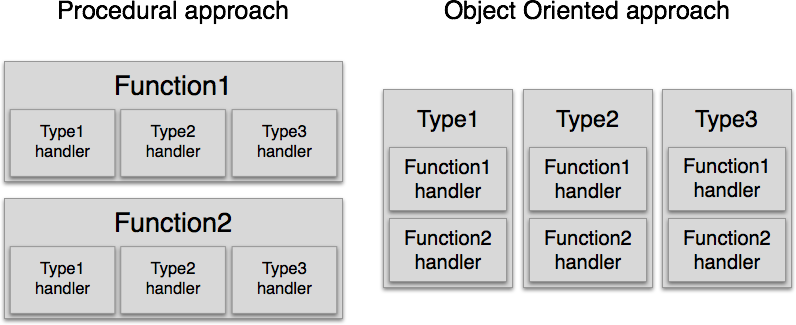
\includegraphics[scale=0.5]{images/approaches.png}
			\caption{Classic and modern approaches}
		\end{center}
		\label{fig:approaches}
	\end{figure}

An example of the difference could be a function to calculate the weight of a car: the classic approach would have a single function with support for all known types of cars; the object-oriented would have one specialized function on each car type. Each approach has pros and cons. If you want to add a car type with the classic approach, you would have to find every place in the code where car-type-specific calculations were made, while with the object approeach, you would only need to implement the functions for the new car type. On the other hand, if you in addition wanted to have a function to calculate the height of a car, in the classic approach, you would need to implement just one function, where in the object-oriented approach, you would have to find all car types, and implement a function for each.

Newer languages with focus on object oriented programming makes the decision of which to use very easy. In pre-object languages, such as C, the choice is a bit harder. The easy answer is to use the classic way, since this is what the language is built for; however, there are ways to build functionality which replicates some object-oriented functions in a procedural way, which makes object composition available.

One other difference between the two approaches is execution speed. The newer, more dynamic ways of programming uses a lot of dynamic lookup at runtime, which has a performance impact, compared to more static programming. If you compare the same code written in C and C++, the C++ code will most likely be a bit slower, since dynamic features like method calls uses runtime table lookups. A more extreme example is languages like JavaScript, which, even when compiled to bytecode, runs at half the speed of the same C program.\footnote{http://ejohn.org/blog/asmjs-javascript-compile-target/}

There isn't a single general answer to, which method is the best to use. It depends on the specific situation. What we can do, is that we can set a general style for the project as a guideline, not a rule. The general style should be prioritized over the other, but if one of them doesn't make sense to use in a situation, the other should be used.

Since most C libraries seem to be using the classic, non-object way, we have chosen to attempt a more modern approach to C programming. The general style guideline for the project is to use object-like thinking when it makes sense: strive to make everything modular and extensible, instead of trying to make it perform.

In the following sections, we will go more in depth with the different design choices in the library.

\section{Memory Management}\label{sec:arch_memory_management}

Manual memory management is often a big hurdle for people coming from garbage collected languages. With the right techniques and code structure, it can become less of a problem, but it's still something that can cause not only headaches during development and debugging, but also commonly causes stability- and security problems when release, if not all bugs are found. This is especially in collections, where programmers are often tempted to just create a static array instead of something that is dynamically expanding, because of the trouble of having to keep track of when you don't need it any more, leading to buffer overflow issues. And, apart from direct code problems, garbage collection is just a convenience that many high-level programmers expects to have. This is why we want our collections to be garbage collected.

Since there is no support for garbage collection in the C runtime, it has to run on top of the standard memory allocation. There are a number of libraries to do this, the most popular of these being the Boehm-Demers-Weiser conservative garbage collector\footnote{\url{http://www.hpl.hp.com/personal/Hans_Boehm/gc/}} (also known just as Boehm's garbage collector), which is used as the garbage collector in Mono and as a leak detector in the Mozilla project. It has replacement functions for malloc and realloc, which will instead allocate memory in heap blocks allocated by the garbage collector, and associate mark-ing bits. For collecting memory, it uses mark-sweep to find unused memory blocks and free them \cite[chap. 10]{Sestoft2012}. Finalizers can also be registered for a block of memory, which could be used to replicate the functionality of deconstructors.

For use in a C program, the mark-sweep method has the advantage of being able to be made conservative. This ensures that there will be no problems in trying to differentiate pointers and integers, since there is no harm done by retaining a block of memory, that isn't in use, but has an integer — which can be interpreted as a pointer, but really is just a value — pointing to it. Non-conservative garbage collectors, such as stop-and-copy, would have to make a choice wether to move the block, and update the potentially false pointer, or garbage collect the memory \cite[chap. 10]{Sestoft2012}.

In regards to performance, the mark-sweep collector can be slow for larger allocations, but is generally fast for smaller ones. Boehm's garbage collector claims to be on-par or faster than regular C memory management for smaller allocations, but slower for larger ones\footnote{As stated in the documentation for GC on the website}.

\section{Data Objects}\label{sec:arch_data_objects}

The most obvious problem we encounter is how to have an insert function, which can insert any kind of object. A collection should be able to contain every type of object, which isn't a problem in object oriented languages, where there is a system of classes and instances, but is a little more tricky in C, since there are multiple distinct type of objects. We will want a function to insert both a char, which is a single-byte stack variable, an int, a multi-byte stack variable, a string, which is a pointer to a block of memory with an unknown size, along with whatever data structure the user has made.

There are multiple approaches to this. One way is to have the user specify an element size when creating the data structure, and any value can then be put into each element, as long as it doesn't exceed the element size. Another way is to make an insert function for each supported data type, so that you would have functions such as \highlight{insert\_int}, \highlight{insert\_float} and \highlight{insert\_string}.

There are some problems with both of these approaches. The first approach prevents the collection from containing different types of objects, if you don't want to get into typecasting when retrieving items. Also just inserting values will not be type-safe, since there will be only one insert function to handle any type. The second approach solves these problems, but this gets back to the classic/dynamic style discussion earlier. We would not be able to add custom data types this way. The only way to insert a custom data structure would be to constantly serialize it to a byte sequence.

The approach we have chosen is to delegate the task of handling different types away from the collections. We will define a data type, which will act as a wrapper for whatever kind of data needed, called \highlight{cc\_object}. Along with making the collections only need to worry about one type of data, the cc\_object can also handle comparison, value equality, data conversion, serialization and hashing, all in an extensible manner.

	\begin{figure}[ht!]
		\begin{center}
			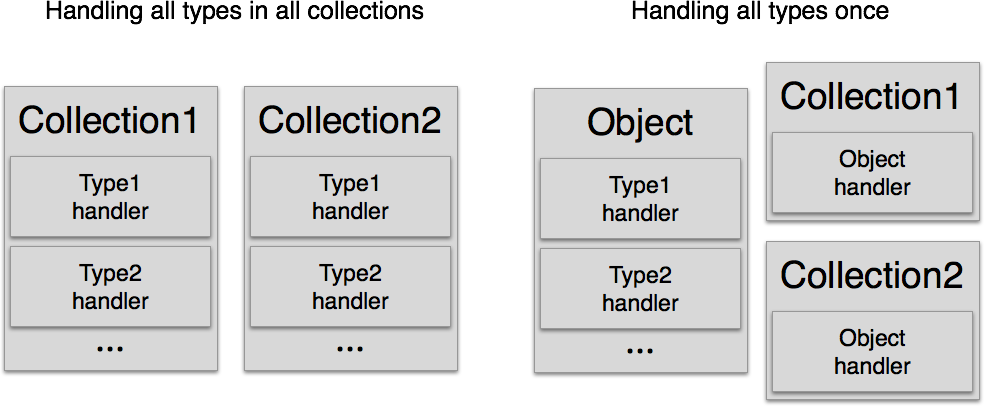
\includegraphics[scale=0.4]{images/types.png}
			\caption{Handling types in a single location}
		\end{center}
		\label{fig:types}
	\end{figure}

The cc\_object works by having a data structure, which supports each item type, and has special insert functions for each. The difference from having a lot of insert functions on the collection is that when you add a new data type, you only have to add one new function to the cc\_object, instead of adding a new function to each collection. This is the same idea as used in Objective-C, where the collection classes cannot contain primitive data types, so numbers gets wrapped in NSNumber instances, and various structures in NSValue instances. If you would save an integer in a collection, you would make an \highlight{NSNumber} with the \highlight{-numberWithInteger:} method, and the other way around call the \highlight{-integerValue} method to get the primitive value back. Likewise, with cc\_objects, you would create a new object with the \highlight{cc\_object\_with\_int} function, and to get the value back, use the \highlight{cc\_object\_int\_value} function. When using custom data types, the user can just make a custom cc\_object initializer method, to keep everything type-safe.

A very useful feature of object-oriented languages, which is difficult to replicate in C, is the concept of interfaces. Suppose that you want to be able to compare two cc\_objects. If they were objects, you would just make a comparable-interface, and have each object-subclass implement a compare method. In C, we'll have to use a slightly different method.

To handle different types of cc\_objects (which in object oriented languages would be to make subclasses of an abstract superclass), we use a string identifier on each object, to indicate its type. The CCollections library has a few built-in types, such as \highlight{cc\_object\_type\_int} and \highlight{cc\_object\_type\_string}, and it is possible to define custom types. Allowing us to identify the type of an object, allows us to get the same result as using an interface. With a function call, a function can be registered as the comparator function for a specific type. When the user calls \highlight{cc\_object\_compare}, the function will first compare the types of the two objects. If they are not the same type, we can already say that they're not equal. If they are, we call that type's comparator function.

With the cc\_object-approach, we have, in normal C code, replicated some of the functionality from more modern languages, making the code more dynamic and extensible.

\section{Collection and enumerator architecture}\label{sec:arch_collections}

We want our collections to be architectured in a way so that they have a common interface for data exchange. We want it to be easy to convert between different data structures, and to get data in and out of the different kinds of collections. We already have a uniform way of storing different data types with our object structures, and we need something like that for our collections.

The way to have all data structures be interchangeable is to have a common structure, that each can convert to and from. In this collection, we have chosen enumerators to be that common data structure. All collections should be able to return an enumerator, and all collections should be able to be created with an enumerator as argument.

The next problem is how to do this in C. In an object oriented language, we would be able to make an enumerable interface, which all collection subclasses could implement. We do not have this feature in C. What we can do have is the ability in incapsulate structures in other structures. This allows us to make something not unlike inheritance from object oriented languages. By defining a \highlight{cc\_enumerable} struct, we can place this inside of a \highlight{cc\_collection} struct to "implement it" in the collection. We will then be able to add function pointers, which each type of collection can override, to provide their own implementation. This approach is necessary for functions to be called automatically by the library. In this case, it's the move next function, which should take a step in the enumeration. Getting an enumerator from a collection is not something that needs to be done automatically, but rather something the user of the library should do, so we don't need to define it this strongly, but rather just ensure that the collections follow a specific style for getting enumerators.

With this approach, a collection can have a method to return an enumerator, and the enumerator will be able to crawl through the objects of the collection by calling that collection's move next function, which it will have, since it incapsulates an enumerable struct.

The approach of using enumerators as an interexchangable collection format allows us to do something else, which is in many other collection libraries, but traditionally would be difficult to implement in C. In C\# and especially many functional languages, you can easily filter, map, sort and take elements from a collection. With the enumerators as a standard "collection", we can implement this functionality as well. We can make functions that takes an enumerator and returns a new, which will then create a chain of move next implementations, where each link can filter out items, map items to different types, or whatever the function does. This allows us very easily create chains of collection modifiers, in a way that is typically only seen in higher level languages.

	\begin{figure}[ht!]
		\begin{center}
			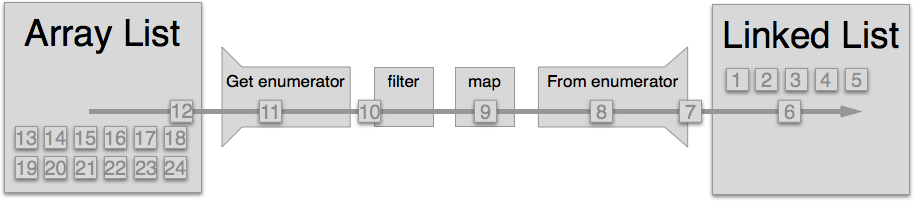
\includegraphics[scale=0.4]{images/enumerators.png}
			\caption{An example of usage of enumerators. We get an enumerator from the array list, which has some filters and mappings, and is then creating a linked list}
		\end{center}
		\label{fig:enumerators}
	\end{figure}

\section{Code Structure}\label{sec:arch_code_structure}

To have a well structured source code is very important in regards to debugging, testing and maintainability of the project. That's why we are strictly following some basic rules regarding structure, information hiding and naming.

One of the most fundamental structural decisions is to enforce information hiding through the idea of the black box: a potentially decoupled interface and implementation, and only exposure of the interface to the user of the module \cite{Gelder2001}. In Java-like languages, you would implement a black box like this with the public and private keywords, for selecting which parts of a class should be exposed, and which should not. In addition, things can be marked as not visible to a user, but visible to the rest of the package. In C, such levels of visibility is implemented with header files. Typically, you will have one header file and one implementation file per black box, with the header file being the public interface. Other projects have a single header file for all public interface code in a library. The one-header-per-module approach is the most common in C, and also what we will use. In addition to this, to implement a package-private like behavior, modules may also have a header file for use internally in the project, which should not be exposed to the user. This allows the user to "leak" some implementation details internally. This should be used for details relating to the internal structure of the project's data structures, not the implementation of the specific algorithm or data structure.

In addition to keeping a minimally exposed interface, it should also be documented with a description of each function, along with pre- and post conditions. See the documentation chapter for more.

% [^headernote]: the one-header-per-library method is mostly used when the product of the project is an API, and not an implementation. An example of this is OpenGL, which is an API implemented differently across platforms, with the whole public interface in the gl.h header file.

\section{API}\label{sec:arch_api}
	One of the problems with a lot of C libraries is the API design. If you don't put some thought into making a consistent and readable interface, it will make the whole project seem messy. Functions will have many paramters which may lead them to be more prone to errors.

	One of the goals in this project is to have consistent and well organized interfaces to our collections. We have made a style guide, that all code should follow, that is inspired both by classic C-style naming and more Java-style method naming.

	We have defined a style guide for both public interfaces and internal function implementations.

	\subsection{Style guide for public interfaces}\label{sec:arch_style_public}
	
		\begin{description}
			\item All names must be in lowercase, with underscores separating each word. To avoid naming collisions, they should be prefixed first with cc for the library, and then the name of the object or module it belongs in (e.g. \highlight{cc\_set} and \highlight{cc\_set\_add()}). Struct names must end in struct, and should be typedef'd to the name without struct (e.g. \highlight{struct cc\_set\_struct} and \highlight{cc\_set}).
			\item All objects must have a constructor function called new (e.g. \\\highlight{cc\_set\_new()}). All other "methods" to this object should take an instance pointer as the first parameter (e.g. \\\highlight{cc\_set\_add(cc\_set *set, cc\_object *obj)}). If the function returns anything through a parameter, it should be at the end of the parameter list. Furthermore, all objects must define a type string as a global constant, whose value should be the name of the object (any prefixes included).
			\item All global constants must be defined in the interface as an extern const pointer, and be implemented in the belonging implementation file (e.g. \highlight{extern const char * const cc\_set\_type}).
			\item No struct should be defined in the public interface. All interaction with the object should be done through functions. The definition of the struct should be in the private or package private interface.
			\item Everything defined in a public interface should have Doxygen documentation.
		\end{description}
	
	\subsection{Style guide for internal implementation}\label{sec:arch_style_internal}
	
		\begin{description}
			\item All object structs must start with a cc collection variable.
			\item In the constructor, the object must register a comparator for its type and specify an
			implementation for enumerator move next in the cc collection variable.
			\item Elements in an implementation file must have the following order: constant definitions, private function declarations, constructor implementation, public function implementations, private function implementations.
		\end{description}
		
\section{Testing}\label{sec:arch_testing}

As noted earlier only some of the libraries encountered in our search on the internet had testing implemented. Some had a few tests per data structure to make sure that the data structure sort-of worked. A few had full-blown test suites with all public functionality tested. A lot of had no tests or no tests checked in to the public source at least.

The library for this project will be using unit tests with coverage of all data structures and all public API functions. This will serve three main goals of the library.

\begin{enumerate}
\item The library is well-tested. Every time a change is made to a data structure or another part of the library, which may affect several data structure, all the tests can be run to check nothing breaks. This dramatically lowers the chance of small bugs creeping in.
\item Tests drive forward implementation. This is also known as Test-Driven Development; TDD for short. Once the general structure of the library has been determined features can be fleshed out by writing the tests first and then the implementation. This will both ensure all API is tested but also that there is no API features that has not been tested.
\item A well tested library will encourage third-party developers, who wish to extend and contribute their code to the library, to write tests for their code. Looking at the existing tests will also make it easier for the developer to write matching tests for their code.
\end{enumerate}

\section{Error handling}\label{sec:arch_error_handling}

Libraries like C\# and Java has native support for Exceptions which makes it really easy for developers to determine whether something went wrong and then take proper actions. Since C doesn't have any native support for handling errors we'll have to deal with them in other ways. There are several approaches to the problem.

\begin{itemize}
	\item Return values (-1, -2, etc. corresponding to an error)
	\item out parameters. functions have a last parameter that will contain an error message or code that must be checked.
	\item callbacks. functions have a callback parameter that takes a function pointer to a function that will be called with a error message or code.
	\item global callbacks. like callbacks but there is only a global function that will be called no matter where the error occurs.
	\item error state. each instance of a data structure holds a state which indicates whether an error has occurred along with an error code or an error message. Developers will have to check to check the error state for each call.
	\item long jump. this can be used to create something like the try..catch pattern.
\end{itemize}

The optimal solution for a project like this would be the last option. With a setjmp/longjmp wrapper and an exception object, we could make something that would very much resemble the try..catch pattern, which is known from newer languages. This approach allows both checking for errors after a single function call, jumping out of a block of code on error, and having a global handler for uncaught exceptions. An example of a try..catch implementation in C is [insert example link and description here].

\chapter{Implementation}

\section{Performance}

The programming language C has a huge asset that makes many developers strive towards it still: performance. The language is statically typed and does not run through a CLR (Common Language Runtime) or VM (Virtual Machine) like C\# and Java does. Everything is compiled directly to bytecode. This means that many developers who write C code often do so because of it's great performance advantage. Thus is performance often a great concern for developers using C when searching for libraries. 

However, the design choices made about this library favors functionality, new concepts and usability over performance. Performance is still as important as ever, but not focused on in this project for two main reasons:

\begin{enumerate}
	\item The overall goal of this project is as mentioned earlier to investigate possible implementations of concepts taken from OO-language collection libraries. These languages have wildly unsimilar qualities, some of which will be mimicked in the implementation of this project, inherently hurting the level of performance that could otherwise be achieved.
	\item While some of the design decisions hinters or dampens performance it would be possible still be possible to optimize them for performance. However, optimizing for and testing performance impacts is a hugely time consumptious task that needs thorough research and investigation. The time needed to be spend on performance optimization is much better spend on investigating implementation of concepts as described in 1.
\end{enumerate}

\section{Data Objects}\label{sec:impl_data_objects}

Our design goal with the item objects is to have them be very simple, yet quite extensible. We have some built in basic functionality, but the idea is that the user of the library can extend it with their own custom data types and functionalities.

The objects does two things: first, it can serialize and de-serialize data; second, it can implement functions to run on the objects. For data serialization, we support three primitive data types: int, float and string (const char *).

\begin{lstlisting}[label=cc_object-serialization,caption=Example of how to serialize an int to and from a cc\_object]
cc_object *number = cc_object_with_int(42);
int in_val = cc_object_int_value(number);
\end{lstlisting}
	
In addition to this, we have initializers for making custom data types with ether a pointer (void *) or a data block with a length. Since we are using garbage collection in the project, there is not need to specify, who "owns" a pointer (i.e. who is responsible for free'ing it), when saving a pointer in a cc\_object. The pointer and data types can be used directly, and just contain whatever data type you want, but the preferred approach is that each custom data type in a project will have their own serialization and de-serialization to and from cc\_objects, which will be implemented with the pointer or data type object. This is also why you have to specify a data string when creating a cc\_object with a pointer or data block. The custom serialization function on a custom data type should have a type string, which is unique to that type, and set it on the cc\_object when serializing. An example of a custom cc\_object serialization function is the one from the cc\_linked\_list object:

\begin{lstlisting}[label=custom-serialization,caption=Example of how to implement custom serialization]
// cc_linked_list.h
extern const char *const cc_linked_list_type;

// cc_linked_list.c
const char * const cc_linked_list_type = "cc_linked_list_type";

cc_object *cc_linked_list_to_object(cc_linked_list *list) {
  return cc_object_with_pointer(list, cc_linked_list_type);
}

cc_linked_list *cc_linked_list_from_object(cc_object *object) {
  return cc_object_pointer_value(object);
}
\end{lstlisting}

\textbf{A note on naming: even though the build-in functions for creating cc\_objects has the naming convention of cc\_object\_with\_<type> and cc\_object\_<type>\_value, custom data types should still follow the style guide and be prefixed with the object name.}\\

In this example we use the pointer type to save the linked list to a cc\_object, since it's quite complex and a lot slower to serialize it to a block of data, and store a copy of it that way. The main difference between the pointer and data block types is that the pointer references the item, while the data block copies the item. Which one to use varies, and it is up to the writer of the specific data type to choose. Optionally both functions for making referenced and copied objects can be implemented. In this case, they should have a different data type string, since they will no longer be comparable.

Apart from using the cc\_objects for saving data, we can, as previously mentioned, implement functionality on top of them. An example of this is the built-in object comparators. The comparator functionality allows us to compare to cc\_objects. To be able to compare objects, we need to have a comparator function for each data type. For this, we have the \highlight{cc\_object\_register\_comparator\_for\_type} function, which takes a type string and a function pointer. When creating a custom cc\_object type, you can implement a custom comparator function, and register it with this function. For comparing two cc\_objects, you use the \highlight{cc\_object\_compare} function. This function will first compare the types of the two objects: if they're not the same type, we can already say that they're not equal. If they are, we will find the comparator function registered for that type, and return the result of that. The CC library comes with comparators for the built-in types already registered.

This shows how to implement dynamic functionality on top of the cc\_objects. The point of doing it this way is that users of the library can create their own functionality like this, just as we do it internally. An example of custom functionality could be a cc\_object to JSON function. If the user want this in his or her program, it's as easy as defining a function prototype, which will encode a cc\_object to a JSON string, and write an implementation for each object type. This way, it would also work recursively: the implementation function for a list type would just need to call the JSON serialization function on all it's contained cc\_objects. When implementing such custom functionality, one would need to write implementations for all object types in the CC library, as well as all custom data types. This works just like extensible classes in an object oriented language, except that it's in completely standard C code.

\section{Code Reuse}\label{sec:impl_code_reuse}

As a side effect of great architectured extensibility of the library it becomes very easy and convenient to reuse code across the library. All data structures of course share the cc\_objects and enumerators code. But data structures can be built as extension of another data structure.

\begin{lstlisting}[label=cc_set-struct,caption=Example of internal code reuse]
struct cc_set_struct {
  cc_collection c;

  cc_linked_list *list;
};
\end{lstlisting}

This is illustrated nicely with \highlight{cc\_set} implementation of a set of unique items. The set data structures is built on top of the \\\highlight{cc\_linked\_list} data structure, reusing all the code for insertion, deletion, enumeration and more. All that the set implementation needs to do is to forward calls to the linked list and provide a new insertion function that checks if an item is already in the linked list. Thus building on the 400+ lines of code long linked list implementation and just providing a mere 140 lines of set implementation code.

\section{Enumerators}

	The enumerators are supposed to be a unified way to loop through elements of a collection. In languages like C\#, their main use is in the foreach loop, which is an easy syntax for looping through a collection. The foreach loop has some advantages over the traditional ways of looping through collections, such as a unified interface (you can have same code for looping over both an array list and a linked list. In the traditional way, you would need a for loop for the array list and a while loop for the linked list), and it's less likely to have bugs (it's common to have one-off errors in code that loops over indexes). While we cannot recreate the foreach (at least without getting into some ugly preprocessor code), we can recreate the functionality.

	An enumerator is in of itself pretty simple. It actually only has two functions: getting the current item, and moving to the next item, and the actual functionality is implemented by the collection being looped. The enumerators doesn't even have a public constructor function; it is each collections responsibility to both declare and implement that. The enumerator is left pretty simple, since it's only supposed to act as an interface to the collections.
	
	\begin{lstlisting}[label=cc_enumerator-struct,caption=The enumerator struct]
	struct cc_enumerator_struct {
		cc_enumerable *enumerable;
		void *data;
		cc_object *current;
	};
	\end{lstlisting}

	When a collection wants to implement support for enumerators, they just need to create a function for getting an enumerator for that specific collection, such as \highlight{cc\_linked\_list\_get\_enumerator}. That function should then return a new enumerator, with the \highlight{move\_next} function pointer set to that collection's move next function. The enumerator's move next function will call that when it needs to move on the next element. The enumerator has two data fields: one is a \highlight{cc\_object}, which should be set to the item that is the current item in the iteration, and which is returned from the \highlight{get\_current} function, the other is just a void pointer, which the collection can use to keep track is its progress. With these few things in place, we can now very easily iterate over collections:
	
	\begin{lstlisting}[label=cc_enumerator-impl-example,caption=Implementation of linked list's get_enumerator]	
	cc_enumerator *cc_linked_list_get_enumerator(cc_linked_list *list) {
	  cc_enumerator *e = cc_enumerator_new(&list->c.enumerable);
	  e->data = NULL;

	  return e;
	}
	\end{lstlisting}

\begin{lstlisting}[label=cc_enumerator-example,caption=Using enumerators in CCollections]
cc_enumerator *e = cc_linked_list_get_enumerator(list);
while (cc_enumerator_move_next(e)) {
  cc_object *obj = cc_enumerator_current(e);
}
\end{lstlisting}

	It should be noted that when creating the enumerator, the current object is not the first object in the collection, but just a null object, and the first object is retrieved with the first call to \highlight{cc\_enumerator\_move\_next}. This is for practical rather than technical reasons, because it allows for a simpler syntax (this way, we can start the while loop right after getting the enumerator. The other way, we would have to validate the return value of \highlight{get\_current}, and then use a do..while).

	The other thing we can use enumerators for, apart from implementing foreach-like iteration, is, as mentioned in the architecture section, to be able to convert between collections, by using the enumerators as an interexchangable collection type. For all collection supporting enumerators, it it possible to get an item-enumerator. All these should also have a designated constructor for taking an enumerator, and filling the collection with the items from that. This would allow us to very easily convert between collection types, no matter how they're implemented. Say that we wanted to convert a collection from an array list to a linked list, we would just use this short piece of code:

\begin{lstlisting}[label=cc_enumerator-new-with,caption=Creating collections with enumerators]
cc_array_list *a_list = ...
cc_enumerator *e = cc_array_list_get_enumerator(a_list);
cc_linked list *b_list = cc_linked_list_new_with_enumerator(e);
\end{lstlisting}

	Another feature we then can implement is running code on each element in an enumerator. This would allow us to do things like filter, map and fold a collection. The way this is implemented is by doing something very much alike what we do in the collections' enumerator functions: we create an enumerator and specify a move next function. The move next function would then call the move next on the "parent" enumerator and setting the parents current object to the childs current object. This would create a completely transparent enumerator, in which we can implement some custom functionality. An example of this is a filter move next function:
	
\begin{lstlisting}[label=cc_enumerator-filter-move_next,caption=Custom enumerator filter]
typedef bool (*cc_enumerator_filter_func)(cc_object *obj);

typedef struct {
	cc_enumerator *parent;
	cc_enumerator_filter_func filter;
} filter_enumerator_data;

bool cc_enumerator_filter_move_next(cc_enumerable *c, cc_enumerator *e) {
  filter_enumerator_data *data = e->data;
  cc_enumerator *parent_e = data->parent;

  // enumerate through the parent enumerator until an item that shouldn't be filtered is found
  while (cc_enumerator_move_next(parent_e)) {
    cc_object *obj = cc_enumerator_current(parent_e);
  
    if (data->filter(obj)) {
      e->current = obj;
      return true;
    }
  }

  return false;
}

cc_enumerator *cc_enumerator_filter(cc_enumerator *e, cc_enumerator_filter_func filter) {
  // create a new enumerator and set the original one as the parent enumerator
	cc_enumerator *en = cc_enumerator_new(cc_enumerable_new(cc_enumerator_filter_move_next));
	filter_enumerator_data *data = GC_malloc(sizeof(filter_enumerator_data));
	data->parent = e;
	data->filter = filter;
	en->data = data;
	return en;
}
\end{lstlisting}    

	With this filter function, we can now apply a filter to any enumerator:

\begin{lstlisting}[label=cc_enumerator-custom-filter,caption=Custom filter example]
bool odd_filter(cc_object *obj) {
  return (cc_object_int_value(obj) % 2 == 1);
}

cc_enumerator *e = cc_enumerator_new(cc_enumerable_new(one_to_ten));
// set the data field to 0
e->data = GC_MALLOC(sizeof(int));
*((int *)e->data) = 0;
cc_enumerator *odd_numbers = cc_enumerator_filter(e, odd_filter);
\end{lstlisting}	

	Other than just being pretty simple to both use and implement, this approach also follows our philosophy of being extendable and customizable: the user of the library can very easily make custom enumerators, just like the default ones. If you, in your project, often needs to reverse collections, you could implement your own function which takes an enumerator, and returns and enumerator that loops through the objects in reverse.

\section{Collections}\label{sec:impl_collections}
	In this section the various collection types implemented in the library will be briefly described. Their description will only be high-level and brief while unique features of the individual collections will be discussed at greater length.

	First a note on the amount and selection of data structures implemented. In this section we will discuss the data structures: \textit{Array List, Linked List, Sorted List, Set, Stack, Queue, Dictionary and Binary Tree}. Although the initial plan was to implement more data structures (see \autoref{sec:vision}) we did not have time for all of them. For more on this refer to the discussion in \autoref{sec:discussion}.

	\subsection{Array List}\label{sec:array_list}
	
	The first collection type we will discuss is the array list. This simple data structure is in reality just a dynamically expanding array. It contains a \highlight{heap} with a fixed capacity for cc\_objects. Once the capacity has been reached the data structure will automatically expands it heap to double its previous size.

\begin{lstlisting}[label=cc_array_list-struct,caption=Internal representation of Array List]
struct cc_array_list_struct {
  cc_collection c;

  cc_object **heap;
  int count;
  int heap_size;
};
\end{lstlisting}

	Above is the internal representation of an array list. Like all other data structures in the library it has a reference to its \highlight{cc\_collection}. The structure also tracks the number of elements currently in the structure (\highlight{count}) and what the currently allocated heap size is (\highlight{heap\_size}). When the structure reaches the heap limit, the next call to the add function will reallocate \highlight{heap} using \highlight{GC\_REALLOC}.

	As the name implies Array List has almost identical time complexity to native arrays. Because arrays are used for storing, and the array doubles its size, the complexity of one insertion at the end of the list is \highlight{$O(1)$}. Insertions at the beginning and the middle is \highlight{$O(n)$} because all subsequent items needs to be moved one item at a time.

	Like all other collections in the library, Array List comes with a standard set of features. In the table below is listed these functions with a snippet of their documentation.
	
	Array list is the only data structure apart from the sorted list that has support for sorting. The only reason other data structures does not have this feature is lack of time to implement it. For more on this see \autoref{sec:discussion}.

	The sorting function of array list uses the well known divide and conquer algorithm, Quicksort. The sorting method has an average case complexity of \highlight{$O(n log n)$} while its worst case is \highlight{$O(n^2)$}. Although that doesn't seem impressive Quicksort has proven to perform better in practice the most other \highlight{$O(n log n)$} algorithms. Quicksort also has the advantage of being easy to implement with in-place partitioning that only requires \highlight{$O(n log n)$} additional space \cite[p. 145]{Algorithms2002}. This algorithm is implemented with array list and is used with calls to \highlight{cc\_array\_list\_sort}.
	
	\subsection{Linked List}\label{sec:linked_list}
	
	The Linked List collection type is as the name indicates a doubly-linked list data structure. The structure store items in node structs and maintains a reference to the first and last item in the list; in the implementation called \highlight{head} and \highlight{tail}.

\begin{lstlisting}[label=cc_linked_list-struct,caption=Internal representation of Linked List]
struct cc_linked_list_struct {
  cc_collection c;

  struct cc_linked_list_node_struct *head;
  struct cc_linked_list_node_struct *tail;

  int length;
};
\end{lstlisting}

	Just as the Array List, the Linked List keeps track of its length (number of items in the list). Each node in the structure contains a reference to the stored \highlight{cc\_object} along with references to the next and previous nodes in the list.
	
\begin{lstlisting}[label=cc_linked_list-struct,caption=Internal representation of Linked List node]
struct cc_linked_list_node_struct {
  cc_object *object;
  struct cc_linked_list_node_struct *next;
  struct cc_linked_list_node_struct *prev;
};
\end{lstlisting}

	Like the Array List, the Linked List has the standard features of \highlight{cc\_linked\_list\_clear}, \highlight{cc\_linked\_list\_contains} and \\\highlight{cc\_linked\_list\_merge}. But unlike any other data structure it has a shorthand function for creating a linked list using an argument list (or, \highlight{va\_list}) of scalar types. The function makes it a lot easier to create a linked list seeded with some initial items without first wrapping them in \highlight{cc\_object}. The function can be used as follows:
	
\begin{lstlisting}[label=cc_linked_list-struct,caption=Creating a linked list with an argument list]
cc_linked_list *a_list = cc_linked_list_new_with_values(cc_object_type_int, 4, 8, 15, 16, 23, 42, CC_END);
\end{lstlisting}

	This features is very similar to what other languages has like Objective-C where you can create an array using the syntax:\\
	\highlight{[NSArray arrayWithObjects: @4, @8, @15, @16, @23, @42]}. Note here that the integers are prefixed the \highlight{@} which makes them into \highlight{NSNumber} instances. The collection type does not take care of the conversion like our implementation does.
	
	\subsection{Sorted List}
	
	Sorted List is the first collection type in the library where code reuse becomes very useful. The structure only has one internal linked list which is used to store the items in.
	
\begin{lstlisting}[label=cc_sorted_list-struct,caption=Internal representation of Sorted List]
struct cc_sorted_list_struct {
  cc_collection c;
  cc_linked_list *data;
};
\end{lstlisting}

	All calls for creating, getting, removing, clearing and enumerating the sorted list is forwarded to the internal linked list using an public functions exposed as the sorted list. The only function that needs to have significant code content is the insertion function. This function then uses an insertion sort algorithm to find the proper place in the linked list to insert the new item. It does so by enumerating the linked list, comparing each item in it with the new item until it finds the correct place. We use a linked list for the implementation because it allows fast modification of the list, which will be done a lot, if it's constantly sorted.
	
	\subsection{Set}
	
	The Set collection is very much alike the Sorted List collection because of its small implementation. Just like the Sorted List it uses a Linked List as internal structure for storing items. Although the Set is much like the Sorted List the interface exposed is a bit different. The Set exposes a lot less features than the Linked List. In the table below is listed the public interface for the Set.
	
	\begin{table}[ht]
		\begin{center}
			\rowcolors{2}{gray!25}{white}
	    \begin{tabular}{| l | l |}
			\hline
			\rowcolor{gray!50}
			\textbf{function}				&		\textbf{Description}															\\ \hline
		    cc\_set\_new            	& Creates a new empty set                         \\ \hline
		    cc\_set\_add            	& Adds an object to the set                       \\ \hline
		    cc\_set\_find           	& Finds the index of an objet in the set          \\ \hline
		    cc\_set\_get            	& Gets an object from a set                       \\ \hline
		    cc\_set\_remove         	& Removes an object from the set                  \\ \hline
		    cc\_set\_clear          	& Removes all objects from the set                \\ \hline
		    cc\_set\_count          	& Get the number of objects in the set            \\ \hline
		    cc\_set\_contains       	& Determines whether an object is in the set      \\ \hline
		    cc\_set\_merge          	& Merges two sets together by adding all objects  \\ \hline
		    cc\_set\_get\_enumerator	& Get an enumerator for the set                   \\ \hline
		    cc\_set\_to\_object     	& Make a cc\_object from the set                  \\ \hline
		    cc\_set\_from\_object   	& Make a set from the cc\_object                  \\ \hline
	    \end{tabular}
			\caption{Public API functions for Set collection}
		\end{center}
	\end{table}
	
	The Set works like the Sorted List by forwarding most calls to the internal Linked List that stores items. Only few functions differ. Adding an object will first check if the object is already in the set using the \highlight{cc\_set\_contains} function. 
	
	\subsection{Stack}
	
	Stack is yet another simple collection type based on an internal Linked List for storing items. The data structures have a small amount of public functions that follow the naming conventions normally associated with a stack. New items can be added to the stack by using \highlight{cc\_stack\_push}, items can be peeked at with \highlight{cc\_stack\_peek} and popped from the stack with \highlight{cc\_stack\_pop}.

	The stack uses the FIFO principle \cite[p. 200]{Algorithms2002}. The Stack uses the pointer to the last item in the linked list as the pointer to the top of the stack. Items pushed to the stack are added to the end of the list and items popped from the stack are removed from the end of the list as well. This gives the benefit of \highlight{$O(1)$} pushes, peeks and pops.
	
	\subsection{Queue}
	
	The Queue collection type also uses Linked lists internally and is extremely similar to the Stack. It also has public functions with naming conventions that matches queues. New items are added to the list with \highlight{cc\_queue\_enqueue} and removed from the queue with \highlight{cc\_queue\_dequeue}. Additionally, the first element in the queue can be peeked at with \highlight{cc\_queue\_peek}.

	The queue uses the pointer to the first item in the linked list as the pointer to the start of the queue. It uses the pointer to the last item in the linked list as the pointer to the end of the queue. Again, a linked list is used because of the fast modification. If we used an array list, each dequeing would need to move the data of all the remaining objects in memory. Items being enqueued are added to the end of the list and items being dequeued are removed from the top of the list. This way the queue follows the FILO principle \cite[p. 200]{Algorithms2002}. Just like the stack the complexity of enqueues, dequeues and peeks are \highlight{$O(1)$}.
	
	\subsection{Dictionary}
	
	The dictionary differs a bit from the other data types, in that it needs two data stores: a set of the keys and some "buckets" for the values. For the keys, it's pretty obvious to use our already implemented set, which works just the way we need it to for our key store. For the value store, we need something for quick lookup from a hash value. For this, we use a simple native C array, because we will, in our initial implementation, just use a fixed heap size. A preferrable extension would be to allow the heap to dynamically expand. Since there may be hash value collisions, the heap will be an array of linked lists. The objects inserted into the dictionary should, if a sufficiently sophisticated hash function is used, spread out evenly in the heap, putting only one object in each linked list. Using an array list with preallocated space for a number of items would be a waste here.

\begin{lstlisting}[label=cc_dictionary-struct,caption=Internal representation of Dictionary]
struct cc_dictionary_struct {
	cc_collection c;
	
	cc_linked_list **heap;
	cc_set *keys;
	int count;
};
\end{lstlisting}

	All the basic dictionary operation implementations are pretty straight forward: adding a value for a key searches for that key, and if it exists overwrites the value, otherwise inserts the new value in the heap and the key in the keys list. Get looks at the place in the heap equal to the hash value of the key. Contains checks if the key exists in the keys list.

	One thing that works a bit different is the handling of enumerators. Getting an enumerator just enumerates over the keys in the dictionary, and the user can just get the value for the current key to get the corresponding item. Creating a dictionary from enumerators is not as simple. It wouldn't make much sense to create a dictionary from a list-enumerator. That's why the dictionary has a constructor function that takes two enumerators: one for the keys and one for the items. This will create the new dictionary with each value from the item-enumerator matched to a key from the key-enumerator.
	
	\subsubsection{Hashing}
	
	In the same way that every object should be able to register a comparator for its type, each object should also be able to specify a hashing function. The library will have built-in functions for hashing (in cc\_hash.h), but for complex data structures, it will be necessary to specify a custom hashing function. This can still use the built in hashing functions for getting the hash of each data field, and then hash those together into a single value. When a data type has registered its hash function with \highlight{cc\_object\_register\_hash\_func\_for\_type}, it's as easy as calling \highlight{cc\_object\_hash} to get the hash of an object of that data type.
	
	As for the hashing algorithm we use, it's a very simple one, and really not a very good one. The ideal solution would to include a hashing library in the project, to be sure that the algorithm is fast and has as few collisions as possible. Some libraries to consider could be CMPH - C Minimal Perfect Hashing Library\footnote{\url{http://cmph.sourceforge.net/}} or gperf - GNU Perfect hashing\footnote{\url{http://www.gnu.org/software/gperf/\#TOCintroduction}}.
	
	\subsection{Binary Tree}
	
	The project has a binary tree implementation. The binary tree is a simple structure, where each node has a left branch and a right branch, and data can be associated with each node. The binary tree structure represents such a node. The only fields it has is references to its parent node, the left branch node, the right branch node, and the associated cc\_object.

\begin{lstlisting}[label=cc_binary_tree-struct,caption=Internal representation of Binary Tree]
struct cc_binary_tree_struct {
	cc_collection c;
	
	cc_object *obj;
	cc_binary_tree *parent;
	cc_binary_tree *left_branch;
	cc_binary_tree *right_branch;
};
\end{lstlisting}

It is also possible to get an enumerator for the tree. The only thing making this a bit more difficult than list structures is, that there is no obvious order, in which the nodes should be returned. To solve this, we have to different enumerators for the binary tree: a depth-first enumerator, as well as a breadth-first enumerator. The way this is implemented is by having two functions for getting an enumerator, as well as two move next functions. Still, when the enumerator wants to move to the next object, it will just call the \highlight{cc\_binary\_tree\_enumerator\_move\_next} function. To figure out which move next function to call, we have saved the enumerator type in the enumerators data field. With this, we can distinguish between the two enumerator types, and call the right move next function.
	

\section{Testing}

	As noted in \autoref{sec:arch_testing} this project will be covering its implementation with functional unit tests. For the implementation of the unit tests a framework called \href{Unity}{https://github.com/ThrowTheSwitch/Unity} has ben chosen. It was picked from a list of 45 competing libraries \footnote{\href{http://en.wikipedia.org/wiki/List\_of\_unit\_testing\_frameworks\#C}{http://en.wikipedia.org/wiki/List\_of\_unit\_testing\_frameworks\#C}}. It features \href{xUnit}{http://en.wikipedia.org/wiki/XUnit} compliant unit tests and is very light weight. This means that it can easily be bundled with library src and does not have to be installed separately from the source like some of the other choices.

	The library features a total of 137 unit tests across all public functions for both the data structures and the cc\_objects and enumerators. The tests can easily be compiled and run straight from the command line using the Makefile. When the command \highlight{make test} is run it will run all unit tests for library and tell how many tests failed or passed.
	
	\begin{figure}[ht!]
		\begin{center}
			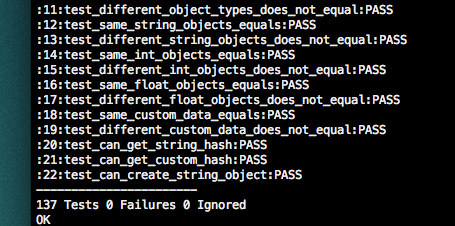
\includegraphics[scale=0.7]{images/test_output.png}
			\caption{Generated test output}
		\end{center}
		\label{fig:generate_test_output}
	\end{figure}
	
	This automation makes it easy to run the tests frequently to ensure that no functionality breaks when working on the library code. The automation could even be taken a step further with tools like Guard that runs the test every time a source code file is saved, notifying the developer of test failures.

\begin{figure}
\begin{lstlisting}[label=test-example,caption=Example of unit test with Unity]
void test_can_create_linked_linked_list_from_array_list(void) {
  cc_array_list *a_list = cc_array_list_new();
  int i;
  for (i = 1; i < 512; i++) {
    cc_array_list_add_last(a_list, cc_object_with_int(i));
  }

  cc_enumerator *e = cc_array_list_get_enumerator(a_list);
  cc_linked_list *b_list = cc_linked_list_new_with_enumerator(e);

  TEST_ASSERT_EQUAL(cc_array_list_length(a_list), cc_linked_list_length(b_list));
  e = cc_array_list_get_enumerator(a_list);
  while (cc_enumerator_move_next(e)) {
    cc_object *obj = cc_enumerator_current(e);
    TEST_ASSERT_EQUAL(true, cc_linked_list_contains(b_list, obj));
  }
}
\end{lstlisting}
\end{figure}
	Above is listed one of the 137 tests of the library illustrating how the Unity framework works. Essentially it boils down to only a few set of macros for determining whether a test fails or succeeds. In the example above the macro \highlight{TEST\_ASSERT\_EQUAL} is used multiple times. The macro takes two arguments where the first is the value expected and the second is the value returned. If the values doesn't match the test will fail.

	\subsection{Coverage}
	
	The Unity framework has a lot of benefits with its lightweight, portability and ease of use but where it falls short is with code coverage. The framework does not include any functionality to determine what percentage of the code is being covered by tests or which paths are not being executed. Some of the frameworks have this functionality but lacks portability or is part of massive libraries that we do not wish to depend upon.

	This means that we cannot make any guarantees that all of the code in the library has been tested. In fact we can almost guarantee that not all code paths have been executed. In turn we can however guarantee that every publicly exposed function in the library has at least one or more test associated with it. Most crucial functions have a lot more.

	A full overview of tests and their results can be found in Appendix A.
	
\section{Documentation}

As mentioned in \autoref{sec:vision} the importance of good documentation for this project is very high. The programming language Java spawned a new era of well documented code with its contestant to the market, JavaDoc. JavaDoc is a documentation generator that takes code documentation and generates browsable HTML documentation for the codes API. JavaDoc defines a syntax that can be used in the comments of code declarations that will help generate well formed API documentation. Other similar libraries have existed before but JavaDoc seemed to really start the movement. Since then other languages has found inspiration and has adopted similar features.

One of the long running contestants is Doxygen. With very similar features to JavaDoc it brings its code documentation syntax to multiple languages. It was originally engineered for C++ but works just as well for other languages like C. Doxygen, like JavaDoc, defines a syntax that can be used to generate browsable API documentation. An example snippet for documentation is listed Below.


\begin{lstlisting}[label=documentation-example,caption=Example of Doxygen comment]
/*! \brief Determines whether an object is in the linked list
 * \param list the linked list to search
 * \param object the object to search the list for
 * \returns true if the object is found in the linked list; otherwise, false */
bool cc_linked_list_contains(cc_linked_list *list, cc_object *object);
\end{lstlisting}


This generates the following entry in the browsable HTML API documentation:

	\begin{figure}[ht!]
		\begin{center}
			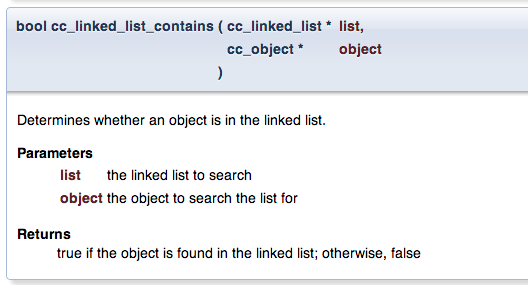
\includegraphics[scale=0.6]{images/doxygen_example.png}
			\label{fig:doxygen_example}
			\caption{Generated documentation example}
		\end{center}
	\end{figure}
	
	Using the Doxygen documentation has multiple benefits that is important to this project. It provides users with great overview of what the library is capable of since all public documentation is there browsable from a single place. It provides them with a single point to look up documentation and find out how a certain collection operates or what kind of functionality is available. It provides users that wish to extend the library with internal documentation that will make it easier to pinpoint what the different internal functions do.
	
	One of the best parts of Doxygen is that it like the unit tests can be fully automated. Running \highlight{make documentation} from the command line will go through all the sources in the library and automatically generate a new HTML documentation ready to be browsed.

	A full overview of all documentation for public functions can be found in Appendix B.

\chapter{Conclusion}

	Our goal with this project was to create a general-purpose collection library for C, that would be simple to include in any project, and be very easy to use, as an alternative to rewriting basic collections from scratch, for each new project. The style of the code should be inspired by modern techniques used in dynamic, object oriented languages, that would make the collections powerful, flexible and easy to extend. We implemented the Boehm-Demers-Weiser conservative garbage collector for automated memory management, to make the code simpler and less errorprone. We made the library flexible by using item objects, which could dynamically be extended with additional functionality. We implemented enumeration, which not only coupled all collections together in a unified format, but also allowed high-level features like filtering, mapping and folding of collections.
	
	In this project, we have back-ported some of the great improvements made by modern languages, to make a starting point for developers using object oriented languages to pick up C, and see, how modernly inspired C code should work. It's a departure from the classic performance-persuing C programs, to a more dynamic code.
	
	
	\section{Discussion}\label{sec:discussion}
	
		Even though we made a lot of progress and implemented a lot of feature in this library we did not get to do all the things that we set out to do from the start. There is also a number of things we learned during the process that we would like to have done differently. We will go over some of these features and problems in this section.
		
		\subsection{Outstanding functionality}
		
			In \autoref{sec:vision} we listed a number of collection types that we planned to implement during this project. Limited by time we faced the decision to focus on implementing all the collection types or to take more inspiration from modern libraries and implemnt features that had not been seen in C before. Instead of implementing all collection types we decided to focus on enumeration, filtering and mapping. The collection types we choce not implement are Sorted Set and Sorted dictionary.\\
			
			In \autoref{sec:linked_list} we demonstrated how we implemented the functionality to create a Linked List using an argument list as seed. This feature makes the creation of collection types much easier. Even though we wished to, we did not get to implement that feature for the rest of the collection types. We did however get to demonstrate how it can be done, which means it will be fairly easy to implement for the rest of the collection types.
			
		
		\subsection{Wish list}\label{sec:wishlist}
			
			Having spent a lot of time figuring out how to properly architecture a modern collection library for C and implemnting such a library with basic collection types leaves us with many features we still wish to implement. Here is a few of the features that we would love to have had implemented but did not have time to.
			
			Since this project is completely open source and hosted with version control on GitHub it is hoped that other developers will contribute. Contributers may take inspiration from this section and implement features that we did not have time to implement.
			
			\begin{itemize}
				\item \textbf{More collection types:} There are still a lot of collection types that could be useful to have in a collection library. Common collection types from other modern libraries that we did not implement are \textit{Hash Tables, Hash Sets, Hash Lists and Priority Queues}.
				\item \textbf{Better sorting:} A more unified interface for sorting collections that would not leave each collection type implementation up to providing its own sorting meachanism. In general more sorted collection types are missing.
				\item \textbf{Test coverage:} Because we chose to use Unity instead of other libraries like Check or CUnit we did not have test code coverage statistics. This would have been a great tool to have for eliminating bugs.
				\item \textbf{Performance testing:} Even though performance never was in focus in this project it would be great to have benchmarks. Just simple test showing the overhead of using our cc\_objects would be great.
			\end{itemize}

		% - What we didn't get to
		% 	- The remaining collection types
		% 	
		% 	- sorting for more collection types
		% 	- collections with argument lists for all collection types
		% - Wish list
		% - Proper use of hashing functions like comparators
		% 	- More collection types
		% 		- Hash tables
		% 		- hash set
		% 		- priority queue
		% 	- Performance testing
		% 		- benchmarking to show the performance impact of our solution
		% 		- being able to pinpoint bottlenecks
		% 	- Test code coverage (we should have picked another library)
		% 	- Better hashing
		% 	- some way to have sorted interface to get a sorted version from an enumerator
		% 	- key/value pair as a cc\_object type

\chapter{Abbreviations \& Definitions}
\begin{acronym}
	\acro{ADT}{Abstract Data Structure}
	\acro{API}{Application Programming Interface}
	\acro{APR}{Apache Portable Runtime,\\ see \url{http://apr.apache.org/}}
	\acro{FIFO}{First In First Out, see \cite[p. 200]{Algorithms2002}}
	\acro{FILO}{First In Last Out, see \cite[p. 200]{Algorithms2002}}
	\acro{GDSL}{The Generic Data Structures Library,\\ see \url{http://home.gna.org/gdsl/}}
	\acro{Glib}{Gnome Library,\\ see \url{https://developer.gnome.org/glib/2.34/}}
	\acro{JavaDoc}{A documentation generation engine developed by Sun for Java}
	\acro{LibDS}{A Portable Data Structures Library,\\ see \url{http://libds.sourceforge.net/doc/index.html}}
	\acro{NPR}{Netscape Portable Runtime,\\ see \url{http://www.mozilla.org/projects/nspr/}}
	\acro{OO}{Object Oriented}
	\acro{SGLib}{A Simple Generic Library for C,\\ see \url{http://sglib.sourceforge.net/}}
\end{acronym}

\nocite{*}
\bibliographystyle{alpha}
\bibliography{report}

\chapter{Appendix}
\appendix
	
\end{document}